\section{The Fourier and Wavelet Transforms}\label{sec:ch2:fourier}

  Computer vision is an extremely difficult task. Pixel intensities in an image are
  typically not very informative in understanding what is in that image.
  These values are sensitive to lighting conditions and camera configurations.
  It would be easy to take two photos of the same scene and get two vectors
  $x_1$ and $x_2$ that have a very large Euclidean distance but to a human,
  would represent the same objects. What is most important in defining an image is
  difficult to define, however, some things are notably more important than
  others. For example, the location or phase of the waves that make up an
  image is much more important than the magnitude of these waves, something
  that is not necessarily true for audio processing. A simple experiment to
  demonstrate this is shown in \autoref{fig:ch2:barbara_morph}.
  \begin{figure}
    \centering
      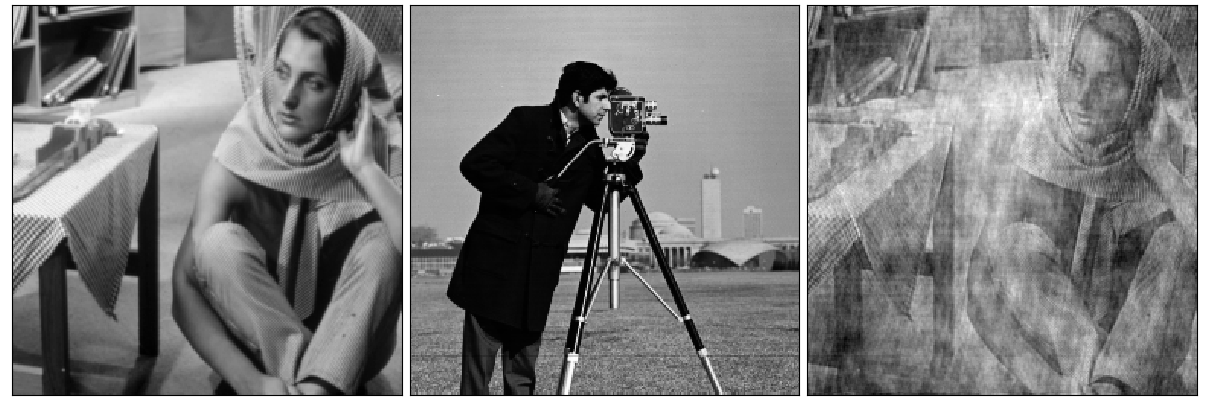
\includegraphics[width=\textwidth]{\imgpath/barbara_mag_swap.png}
      \mycaption{Importance of phase over magnitude for images}
        {The phase of the Fourier transform of the first image is combined with
        the magnitude of the Fourier transform of the second image and
        reconstructed. Note that the first image has entirely won out and
        nothing is left visible of the cameraman.}
      \label{fig:ch2:barbara_morph}
  \end{figure}

\subsection{The Fourier Transform}
For a signal $f(t) \in L_2(\reals)$ (square summable signals), the \emph{Fourier
transform} is defined as:
\begin{equation}
  F(\omega) = \int_{-\infty}^{\infty} f(t) e^{-j\omega t} dt
\end{equation}
This can be extended to two dimensions for signals $f(\xy) \in L_2(\reals[2])$:
\begin{equation}
  F(\ww) = \int_{-\infty}^{\infty}\int_{-\infty}^{\infty} f(\xy) e^{-j\ww^t \xy} d\xy = \langle f(\xy),\ e^{j\ww^t \xy} \rangle
\end{equation}

The Fourier transform is an invaluable signal expansion, as viewing a signal in
the frequency space offers many insights, as well as affording many very useful
properties (most notably the efficiency of convolution as a product of Fourier
transforms). While it is a mainstay in signal processing,
it can be a poor
feature descriptor due to the infinite support of its basis functions - the
complex sinusoids $e^{j\ww^t u}$. If
a single pixel changes in the input it can change all of the
Fourier coefficients. As natural images are generally non-stationary, we need
to be able to isolate frequency components in local regions of an image, and
not have this property of global dependence. To achieve a more local Fourier
transform we can use the short time (or short space) Fourier Transform (STFT) or the
continuous wavelet transform (CWT). The two are very similar and mainly differ in the
way they handle the concept of `scale'. We will only discuss the CWT in this review,
but for an excellent comparison of the two, we recommend \cite[Chapter~1]{antoine_two-dimensional_2004}.

% The Fourier transform does have one nice property, however, in that the magnitude of
% Fourier coefficients are invariant to global translations, a nuisance
% variability. We explore this theme more in our review of the Scattering
% Transform by \Mallat in \autoref{ch:scatternets}.

\subsection{The Continuous Wavelet Transform}
The \emph{continuous wavelet transform}, like the Fourier Transform, can be used
to decompose a signal into its frequency components. Unlike the Fourier
transform, these frequency components can be localized in space. To
achieve this, we need a bandpass filter, or \emph{mother wavelet}
$\psitd$\footnote{We use upright $\psiod, \phiod$ to distinguish 1-D wavelets
from their 2-D counterparts $\psitd, \phitd$} such that:
\begin{equation}
  \int_{-\infty}^{\infty} \psitd(\xy) d\xy = \Psi(0) = 0\label{eq:ch2:admissibility}
\end{equation}
Any function that has sufficient decay of energy with frequency and satisfies
\eqref{eq:ch2:admissibility}, is said to satisfy the \emph{admissibility condition}.

As we are working in 2-D for image processing, consider rotations, dilations, and
shifts of this function by $\theta\in [0,2\pi],\ a>0,\ \bmu{b} \in \reals[2]$ respectively, where
\begin{align}
  \text{Rotation: } & R_{\theta}x(\xy) = x(r_{-\theta}\xy) \label{eq:ch2:rot}\\
  \text{Dilation: } & D_{a}x(\xy) = \frac{1}{a} x\left(\frac{\xy}{a}\right) \label{eq:ch2:di}\\
  \text{Translation: } & T_{\bmu{b}}x(\xy) = x(\xy - \bmu{b}) \label{eq:ch2:tr}
\end{align}
where $r_\theta$ is the 2-D rotation matrix. Now consider shifts, scales and
rotations of our bandpass filter
\begin{equation}
  \psitd_{\bmu{b},a, \theta}(\xy) = \frac{1}{a}\psitd \left(\frac{r_{-\theta}\left(\xy -
  \bmu{b}\right)}{a} \right) \label{eq:ch2:2d_shifts}
\end{equation}
which are called the \emph{daughter wavelets}. The 2-D CWT of a signal $x(\xy)$ is defined as
\begin{equation}
  CWT_x(\bmu{b}, a, \theta) = \int_{-\infty}^{\infty} \psitd^*_{\bmu{b}, a,
  \theta}(\xy) x(\xy) d\xy = \langle \psitd_{\bmu{b}, a, \theta}(\xy),\ x(\xy)
  \rangle \label{eq:ch2:cwt}
\end{equation}

\subsubsection{Properties}
The CWT has some particularly nice properties, such as \emph{covariance}
under the three transformations \eqref{eq:ch2:tr}-\eqref{eq:ch2:rot}:
\begin{align}
  R_{\theta_0}x & \rightarrow CWT_x\left(r_{-\theta_0}\bmu{b}, a, \theta + \theta_0 \right)  \\
  D_{a_0}x & \rightarrow CWT_x\left(\bmu{b}/a_0, a/a_0, \theta \right) \\
  T_{\bmu{b}_0}x & \rightarrow CWT_x\left(\bmu{b}-\bmu{b}_0, a, \theta \right)
\end{align}
Most importantly, the CWT is now localized in space, which distinguishes it from the
Fourier transform. This means that changes in one part of the image will not
affect the wavelet coefficients in another part of the image, so long as the
distance between the two parts is much larger than the support region of the
wavelets you are examining.

\subsubsection{Inverse}
The CWT can be inverted by using a \emph{dual} function $\tilde{\psitd}$. There
are restrictions on what dual function we can use, namely the dual-wavelet pair
must have an admissible constant $C_\psitd$ that satisfies the
cross-admissibility constraint \cite{holschneider_pointwise_1991}. Assuming
these constraints are satisfied, we can recover $x$ from $CWT_x$.
% by:
% \begin{equation}
  % x(\xy) = \frac{1}{C_\psitd} \int \int \int \frac{1}{a^3}CWT_x(\bmu{b}, a, \theta)
  % \tilde{\psitd}_{\bmu{b}, a, \theta}\ d\bmu{b} da d\theta \label{eq:ch2:invcwt}
% \end{equation}

\subsubsection{Interpretation}
As the CWT is a convolution with a zero mean function, the wavelet coefficients are only
large in the regions of the parameter space $(\bmu{b}, a, \theta)$ where
$\psitd_{\bmu{b}, a, \theta}$ `match' the features of the signal. As the wavelet
$\psitd$ is well localized, the energy of the coefficients $CWT_x$ will be concentrated
on the significant parts of the signal.

For an excellent description of the properties of the CWT in 1-D we recommend
\cite{vetterli_wavelets_2007} and in 2-D we recommend
\cite{antoine_two-dimensional_2004}.

\subsection{Discretization and Frames}
The CWT is highly redundant. We have taken a 2-D signal and expressed it in 4
dimensions (2 offset, 1 scale and 1 rotation). In reality, we would like to sample the space
of the CWT in an efficient manner. We would ideally like to fully
retain all information in $x$ (be able to reconstruct $x$ from the samples)
while sampling over $(\bmu{b}, a, \theta)$ as little as possible to avoid
redundancy. To understand how to do this we must briefly talk about frames.
% Consider a family of wavelets $\left{ \phiod_{\bmu{b}_{\nn}, a_j, \theta_k}
% \right} $, then the integral in \eqref{eq:ch2:invcwt} is then replaced with a sum.
% \begin{equation}
  % CWT_x{\bmu{b}_\nn, a_j, \theta_k} = \sum_{\nn, j, k}
% \end{equation}
% This naturally leads to a discussion of frames.

A set of vectors $ \phi = \{ \varphi_i \}_{i \in I}$ in a Hilbert space
$\mathbb{H}$ is a \emph{frame} if there exist two constants $0 < A\leq B <
\infty$ such that for all $x \in \mathbb{H}$:
\begin{equation}
  A||x||^2 \leq \sum_{i\in I} |\langle x, \varphi_i \rangle|^2 \leq B ||x||^2
  \label{eq:ch2:frame_bounds}
\end{equation}
with $A, B$ called the \emph{frame bounds} \cite{kovacevic_introduction_2008}.
The frame bounds relate to the issue of stable reconstruction. In particular, no
vector $x$ with $||x||>0$ should be mapped to 0, as this would violate the bound
on $A$ from below. This can be interpreted as ensuring our set $\phiod$ covers the
entire frequency space. The upper bound ensures that the transform
coefficients are bounded.

Any finite set of vectors that spans the space is a frame. An orthonormal basis
is a commonly known non-redundant frame where $A=B=1$ and $|\varphi_i|=1$ (e.g.\ the Discrete
Wavelet Transform or the Fourier Transform). Tight frames are frames where $A=B$
and Parseval tight frames have the special case $A=B=1$. It is possible to have
frames that have more vectors than dimensions, and this will be the case with
many expansions we explore in this thesis.

If $A=B$ and $|\varphi_i| = 1$, then $A$ is
the measure of the redundancy of the frame. Of course, for the orthogonal basis,
$A=1$ when $|\varphi_i|=1$ so there is no redundancy. For the 2-D $\DTCWT$ which we
will see shortly, the redundancy is 4.

\subsubsection{Inversion and Tightness}
\eqref{eq:ch2:frame_bounds} specify the constraints that make a frame
representation invertible.
The tighter the frame bounds, the more easily it is to invert the signal.
This gives us a guide to choosing the sampling grid for the CWT.

One particular inverse operator is the \emph{canonical dual frame}.
If we define the frame operator $S = \Phi\Phi^*$ then the canonical dual
of $\Phi$ is defined as $\tilde{\Phi} = \left\{ \tilde{\varphi}\right\}_{i \in I}$
where:
\begin{equation}
  \tilde{\varphi}_i = S^{-1}\varphi_i
\end{equation}
then from \cite{kovacevic_introduction_2008} we have:
\begin{equation}
  x = \sum_{i\in I} \langle x, \varphi_i \rangle \tilde{\varphi}_i = \sum_{i\in I}
  \langle x, \tilde{\varphi}_i \rangle \varphi_i
\end{equation}
If a frame is tight, then so is its dual.

\subsection{Discrete Wavelet Transform}\label{sec:ch2:dwt_problems}
  \begin{figure}
    \centering
    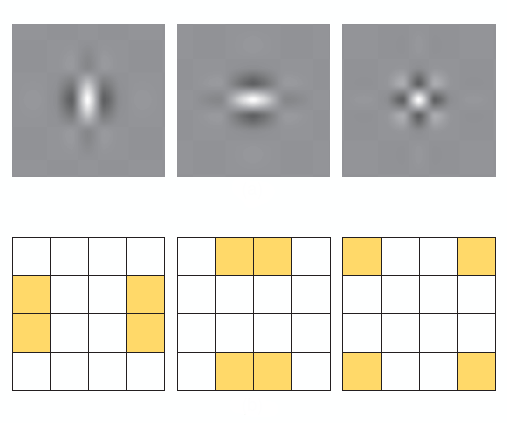
\includegraphics[width=0.5\textwidth]{litreview/images/dwt_wavelets.png}
    \mycaption{Typical wavelets from the 2-D separable DWT\@}{Top: Wavelet point
      spread functions for $\psitd^v$ (low-high), $\psitd^h$ (high-low), and
      $\psitd^d$ (high-high) wavelets. High-high wavelets are in a checkerboard
      pattern, with no favoured orientation. Bottom: Idealized support of the
      spectra of each of the wavelets. Image is taken from
      \cite{selesnick_dual-tree_2005}.}
      \label{fig:ch2:dwt_wavelets}
  \end{figure}
  % \begin{quote}
    % Always operate at the slowest possible sample rate.
  % \end{quote}

  \eqref{eq:ch2:2d_shifts} gave the equation for the daughter wavelets in 2-D,
  in 1-D at scales $a=2^{j}, j \in \integers$, and translations $b = 2^j l,\ l \in \integers$, this is simply:
  \begin{equation}
    \psiod_{j, l}(t) = \frac{1}{\sqrt{a}} \psiod\left(\frac{t-b}{a}\right) = 2^{-j/2} \psiod\left(2^{-j}t- l \right)
  \end{equation}
  where we have chosen to redefine the dilation parameter $a$ in terms of a scale
  factor $j$. As $j$ increases, we move to \emph{coarser} scales.

  The 2-D DWT has one scaling function and three wavelet functions, composed of
  the product of 1-D wavelets in the horizontal ($u_1$) and vertical ($u_2$) directions:
  \begin{align}
    \phitd(\xy) &= \phiod(u_1)\phiod(u_2) \label{eq:ch2:dwt1}\\
    \psitd^h(\xy) &= \phiod(u_1) \psiod(u_2) \\
    \psitd^v(\xy) & = \psiod(u_1) \phiod(u_2) \\
    \psitd^d(\xy) & = \psiod(u_1) \psiod(u_2) \label{eq:ch2:dwt4}
  \end{align}
  with $h, v, d$ indicating the sensitivity to horizontal, vertical and diagonal
  edges. The point spread functions for the wavelet functions are shown in
  \autoref{fig:ch2:dwt_wavelets}.

  For the four equations above \eqref{eq:ch2:dwt1} -- \eqref{eq:ch2:dwt4},
  define the daughter wavelets as:
  \begin{align}
    \phitd^j_{lm}(\xy) &= \phiod_{j,l}(u_1)\phiod_{j,m}(u_2) \\
    \psitd^{h,j}_{lm}(\xy) &= \phiod_{j,l}(u_1) \psiod_{j,m}(u_2) \\
    \psitd^{v,j}_{lm}(\xy) & = \psiod_{j,l}(u_1) \phiod_{j,m}(u_2) \\
    \psitd^{d,j}_{lm}(\xy) & = \psiod_{j,l}(u_1) \psiod_{j,m}(u_2)
  \end{align}
  for $l,m \in \integers$ where $l,m$ define horizontal
  and vertical translation. We can then get an orthonormal
  basis with the set $\{ \phitd^j_{lm}, \psitd^{h,j}_{lm}, \psitd^{v,j}_{lm}, \psitd^{d,j}_{lm} \}_{j,l,m}$.
  The wavelet coefficients at a chosen scale and location can then be found by
  taking the inner product of the signal $x$ with the daughter wavelets.

  % A signal $x \in L_2(\reals[2])$ is represented at resolution $2^j$ by the
  % function $x_j = a_j + \sum_\alpha d^\alpha_j$, where:
  % \begin{align}
    % a_j &= \sum_
  % \end{align}

  \subsubsection{Shortcomings}
  The Discrete Wavelet Transform (DWT) is an orthogonal basis. It is a natural
  first signal expansion to consider when frustrated with the limitations of the
  Fourier transform. It is also a good example of the limitations of
  non-redundant transforms, as it suffers from several drawbacks:
  \begin{itemize}
    \item The DWT is sensitive to the zero crossings of its wavelets.
      We would like singularities in the input to yield large wavelet
      coefficients, but this may not always be the case.
      % if they fall at a zero crossing of a wavelet, the output can be small.
      See \autoref{fig:ch2:dwt_zero_crossing}.
    \item They have poor directional selectivity. As the wavelets are purely
      real, they have passbands in all four quadrants of the frequency plane.
      While they can pick out edges aligned with the frequency axis, they are
      not specific to other orientations. See \autoref{fig:ch2:dwt_wavelets}.
    \item They are not shift-invariant - small shifts greatly
      perturb the wavelet coefficients. \autoref{fig:ch2:dwt_zero_crossing} shows
      this for the centre-left and centre-right images.
      % \autoref{fig:ch2:dtcwt_shift_invariance} (right) also shows this.
  \end{itemize}

  The lack of shift-invariance and the possibility of low outputs at
  singularities is a price to pay for the critically sampled property of the
  transform. This shortcoming can be overcome with the undecimated DWT
  \cite{mallat_wavelet_1998,coifman_translation-invariant_1995},
  but it comes with a heavy computational and memory cost.

  \begin{figure}
    \centering
      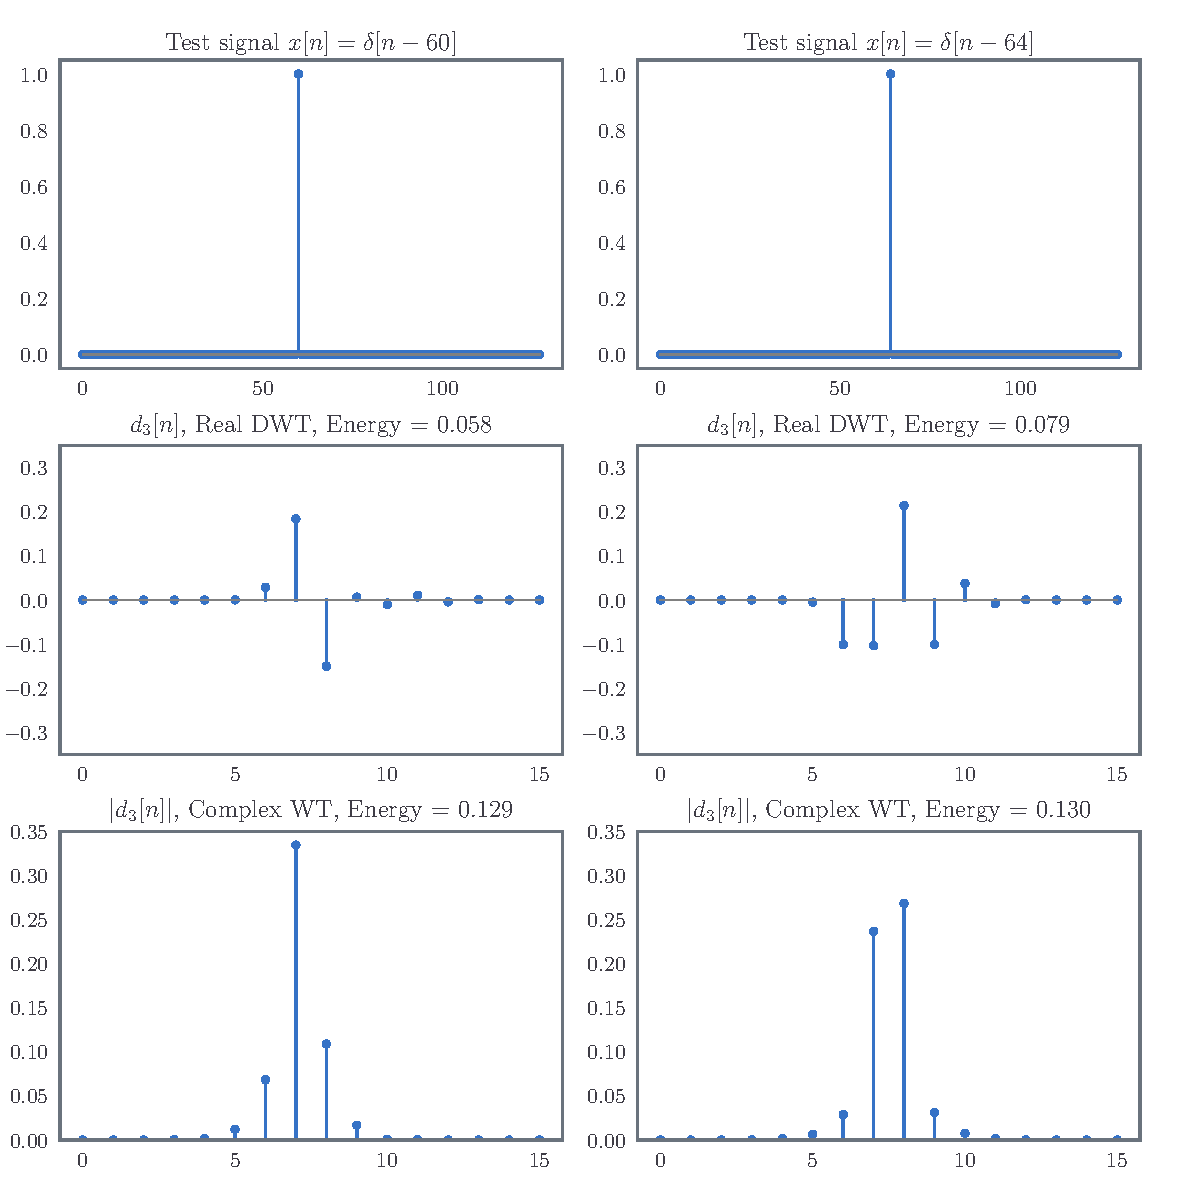
\includegraphics[width=\textwidth]{litreview/images/dwt_zero_crossing.pdf}
      \mycaption{Sensitivity of DWT coefficients to zero crossings and small
        shifts}{Two impulse signals $\delta(n-60)$ and $\delta(n-64)$ are
        shown (top), as well as the wavelet coefficients for scale $j=3$ for the DWT (middle) and
        for the $\DTCWT$ (bottom). In the middle row, not only are the coefficients very different
        from a shifted input, but the energy has almost doubled. As the DWT is an orthonormal
        transform, this means that this extra energy has come from other scales. In comparison, the
        energy of the magnitude of the $\DTCWT$ coefficients has remained far more constant, as has the
      shape of the envelope of the output. Image adapted from \cite{selesnick_dual-tree_2005}.}
      \label{fig:ch2:dwt_zero_crossing}
  \end{figure}

\subsection{Complex Wavelets}\label{sec:ch2:complex_wavelets}
  Fortunately, we can improve on the DWT with complex wavelets, as they can
  solve these new shortcomings while maintaining the desired localization
  properties the Fourier transform lacked.

  The Fourier transform does not suffer from a lack of directional selectivity
  and shift-variance because its basis functions are derived from complex
  sinusoids\footnote{We have temporarily switched to 1D
  notation here as it is clearer and easier to use, but the results still hold
  for 2-D.}:
  \begin{equation}
    e^{j\omega t} = \cos(\omega t) + j\sin(\omega t)
  \end{equation}
  whereas the DWT's basis functions are based on only the real
  sinusoid, $\cos(\omega t)$. As $t$ moves along the real line, the phase of the
  Fourier coefficients change linearly, while their magnitude remains constant. In
  contrast, as $t$ moves along the real line, the sign of the real coefficient
  flips between -1 and 1, and its magnitude is a rectified sinusoid.

  The nice properties of the complex sinusoids come from the fact that the
  cosine and sine functions of the Fourier transform form a Hilbert pair and
  together constitute an analytic signal.

  We can achieve these nice properties if the mother wavelet for our wavelet
  transform is analytic:
  \begin{equation}
    \psiod_{c}(t) = \psiod_{r}(t) + j\psiod_{i}(t) \label{eq:ch2:complex_wavelet}
  \end{equation}
  where $\psiod_{r}(t)$ and $\psiod_{i}(t)$ form a Hilbert pair (i.e.,\ they are
  $90\degs$ out of phase with each other).

  There are a number of possible ways to do a wavelet transform with complex
  wavelets. We examine two in particular: a Fourier-based, sampled CWT using
  Morlet wavelets, and the Dual-Tree Complex Wavelet Transform ($\DTCWT$)
  developed by Kingsbury \cite{kingsbury_wavelet_1998, kingsbury_dual-tree_1998,
  kingsbury_dual-tree_1998-1,  kingsbury_image_1999, kingsbury_shift_1999,
  kingsbury_dual-tree_2000, kingsbury_complex_2001, selesnick_dual-tree_2005}.

  We look at the Morlet wavelet transform because it is used by
  Mallat et.\ al.\ in their scattering transform
  \cite{bruna_classification_2011, bruna_invariant_2013, bruna_scattering_2013,
  oyallon_generic_2013, oyallon_deep_2015, sifre_rotation_2013,
  sifre_rigid-motion_2014, sifre_rigid-motion_2014-1, sifre_scatnet_2013}.
  We believe the $\DTCWT$
  several advantages over the Morlet based implementation, and has been the
  basis for most of our work.

Let us write the wavelet transform of an input $x$ as
\begin{equation}
  \mathcal{W}x = \left\{x \ast \phitd_J, x \ast \psitd_{\lambda} \right\}_{\lambda} \label{eq:ch2:wave2}
\end{equation}
where $\lambda = (j,k)$ with $j\in \{1, 2,\ldots J\}$ indexing the
scale\footnote{We try to number everything from zero in this thesis, but number
$j$ from 1 as is the practice in \cite{kingsbury_complex_2001,
selesnick_dual-tree_2005}.} and $k \in \{0, 1, \ldots K-1\}$ indexing the
orientations of the chosen wavelet transform, whether it be the $\DTCWT$ or
Morlet transform.

\subsection{Sampled Morlet Wavelets}\label{sec:ch2:morlet_fourier}
  % Just need to review in Vetterli, how to do FFT based sampling of the CWT.
  The wavelet transform used by Mallat et.\ al.\ in their scattering transform is an efficient
  implementation of the Gabor Transform.  While the Gabor wavelets have the best
  theoretical trade-off between spatial and frequency localization, they have a
  (usually small) non-zero mean.  This violates \eqref{eq:ch2:admissibility} making them
  inadmissible as wavelets. Instead, the Morlet wavelet has the same shape, but
  with an extra degree of freedom chosen to set $\int \psitd (\bmu{u}) d\bmu{u}
  =0$. This wavelet has equation (in 2-D):
  \begin{equation}
    \psitd(\bmu{u}) = \frac{1}{2\pi\sigma^2} {(e^{i\bmu{u}^t\bm{\xi}} - \beta)}
                     e^{-\frac{|\bmu{u}|^2}{2\sigma^2}}
    \label{eq:ch2:morlet}
  \end{equation}
  where $\beta$ is this extra degree of freedom, and usually $\beta\ll 1$.
  $\sigma$ is the size of the gaussian window and $\bm{\xi}$ is the
  approximate location of the peak frequency response in the Fourier plane, with
  $-\pi \leq \xi_1, \xi_2 \leq \pi$.

  \citeauthor{bruna_invariant_2013} \cite{bruna_invariant_2013} add a further
  additional degree of freedom in their original design by allowing for a
  non-circular Gaussian window over the complex sinusoid, which gives control
  over the angular resolution of the final wavelet. This makes \eqref{eq:ch2:morlet}:
  \begin{equation}
    \psitd(\bmu{u}) = \frac{\gamma}{2\pi\sigma^2}{(e^{i\bmu{u}^t\bm{\xi}} - \beta)}
                  e^{-\bmu{u^t}\Sigma^{-1}  \bmu{u}}
    \label{eq:ch2:morlet_slant}
  \end{equation}
  Where
  $$\Sigma^{-1} = \left[ \begin{smallmatrix}
      \frac{1}{2\sigma^2} & 0 \\
      0 & \frac{\gamma^2}{2\sigma^2}
      \end{smallmatrix} \right] $$
  The effects of modifying the eccentricity parameter $\gamma$ and the window size
  $\sigma$ are shown in \autoref{fig:ch2:morlet_filters}. A full family of
  Morlet wavelets at varying scales and orientations is shown in
  \autoref{fig:ch2:morlet_littlewood_paley}.
  % To have a full two
  % dimensional wavelet transform, we need to rotate this mother wavelet by angle
  % $\theta$ and scale it by $j/Q$, where $Q$ is the number of scales per octave
  % (usually 1 in image processing).

  % This can be done by doing the following
  % substitutions in \eqref{eq:ch2:morlet_slant}:
  % \begin{align*}
    % R_{\theta}& = \left[ \begin{smallmatrix}
                    % \cos(\theta) & -\sin(\theta) \\
                    % \sin(\theta) & \cos(\theta)
                  % \end{smallmatrix} \right] \\
    % \bmu{u}_{\theta} & =  R_{-\theta} \bmu{u} \\
    % \sigma_j & =  2^{\frac{j-1}{Q}} \sigma \\
    % \xi_j & =  \frac{\xi}{2^{\frac{j-1}{Q}}}
  % \end{align*}
  % We can combine these two variables into a single coordinate
  % \begin{equation}
    % \lambda = (\theta, j/Q)
  % \end{equation}
  % We can now scale and rotate this mother wavelet:
  % \begin{equation}
    % \psi_{\lambda}(\bmu{u}) = 2^{-j/Q}\psi(2^{-j/Q}R_{\theta}^{-1} \bmu{u})
  % \end{equation}
  \begin{figure}
    \begin{center}
      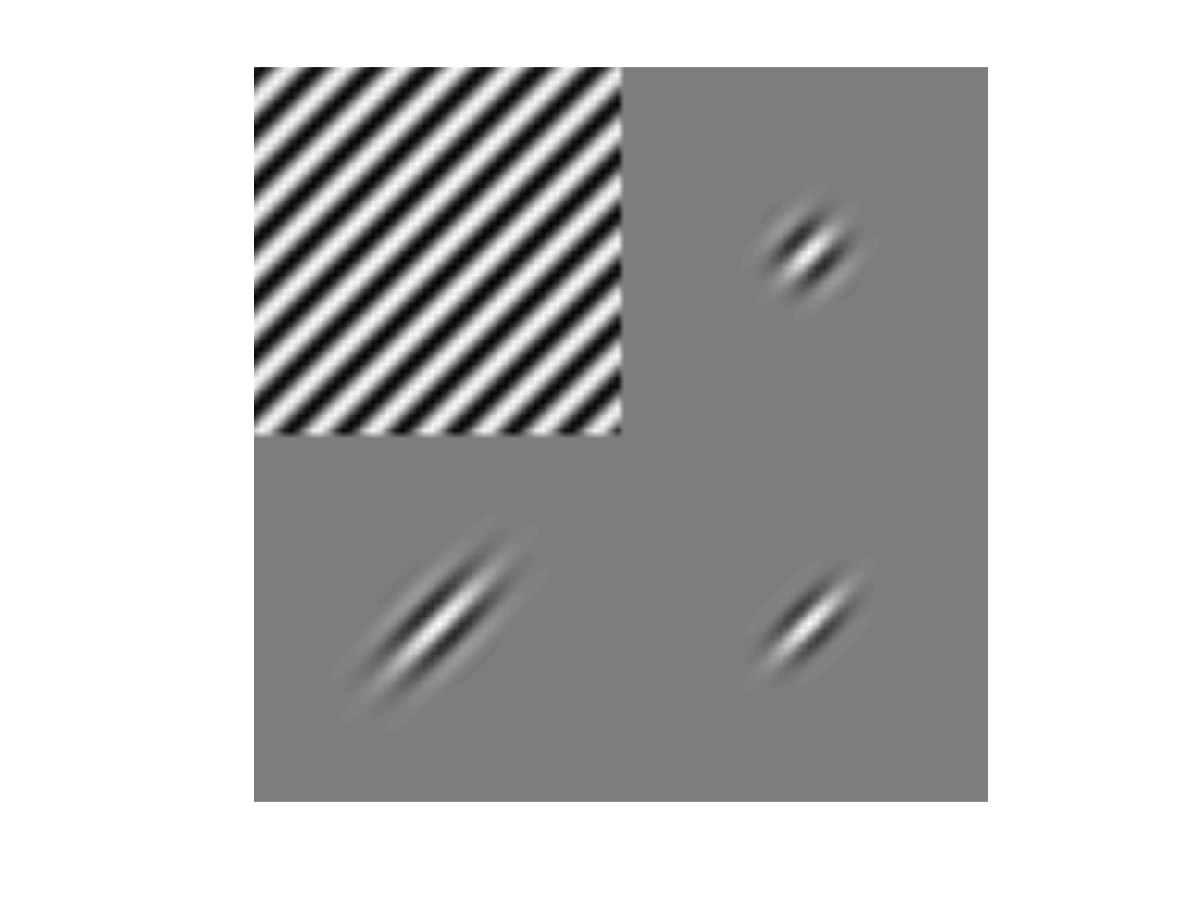
\includegraphics[height=6cm]{\imgpath/morlet_filters.png}
      \mycaption{Single Morlet filter with varying slants and window sizes}
              {Top left --- $45\degs$ plane wave (real part only). Top right --- plane wave with
              $\sigma=3,\gamma=1$. Bottom left --- plane wave with $\sigma=3,\gamma=0.5$. Bottom
            right --- plane wave with $\sigma=2,\gamma=0.5$.}
      \label{fig:ch2:morlet_filters}
    \end{center}
  \end{figure}
  % \begin{figure}
    % \begin{center}
      % \makebox[\textwidth][c]{%
        % 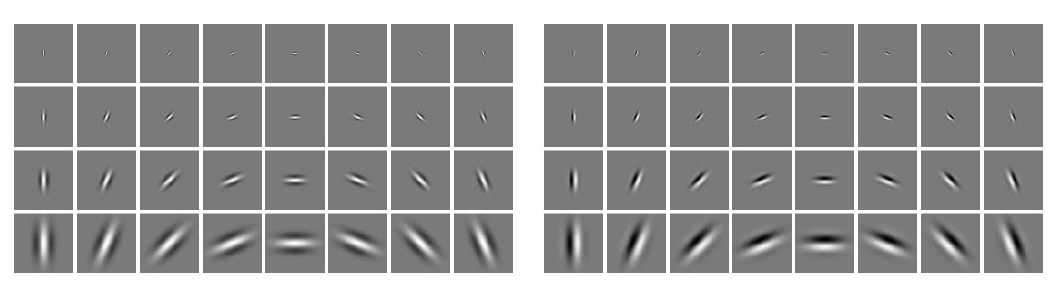
\includegraphics[width=1.1\textwidth]{\imgpath/morlet_wavelets_full.png}
      % }
      % \mycaption{The full dictionary of Morlet wavelets used by Mallat}
              % {The real filters are on the left and the imaginary on the right. The first row
              % correspond to scale $j=1$, increasing up to $j=4$. The first column corresponding to
            % $\theta = 0$, rotating through $\pi/8$ up to the eighth column of $7\pi/8$,
          % $\gamma=1/2$.}
      % \label{fig:ch2:morlet_wavelets_full}
    % \end{center}
  % \end{figure}

\subsubsection{Tightness and Invertibility}
Recall our definition of the wavelet transform $\mathcal{W}$ from \eqref{eq:ch2:wave2}.
Assuming the transform is bounded, we can always scale it so that it satisfies
Plancherel's equality
\begin{equation}
  \norm{\mathcal{W}x} = \norm{x}
\end{equation}
which is a nice property to have for invertibility, as well as for analysing
how different signals get transformed (e.g.\ white noise versus standard
images). Scaling the transform changes the upper bound $B$ in \eqref{eq:ch2:frame_bounds}
to 1 and makes the lower bound $A = 1-\alpha$, where $\alpha$ is a measure of how
non-tight a frame is.

Using the capital notation to denote the Fourier transform, define the function
$A(\ww)$ to be the coverage each wavelet family has over the frequency plane:
\begin{equation}
  A(\ww) = {|\Phi_J(\ww)|}^2 + \sum_{\lambda} {|\Psi_{\lambda}(\ww)|}^2
  \label{eq:ch2:lwood_paley}
\end{equation}
For a unit norm input $||x||^2 = 1$ and scaled wavelets, we can now change
\eqref{eq:ch2:frame_bounds} to be:
\begin{equation}
  1-\alpha \leq A(\ww) \leq 1
\end{equation}
  If $A(\ww)$ is ever close to 0, then there is not a good coverage of the frequency plane
  at that location.
  \autoref{fig:ch2:morlet_littlewood_paley} shows the frequency coverage of a few
  sample grids over the CWT parameters used by Mallat. Invertibility is possible, but not
  guaranteed for all configurations.

  \begin{figure}
    \centering
    \makebox[\textwidth][c]{%
      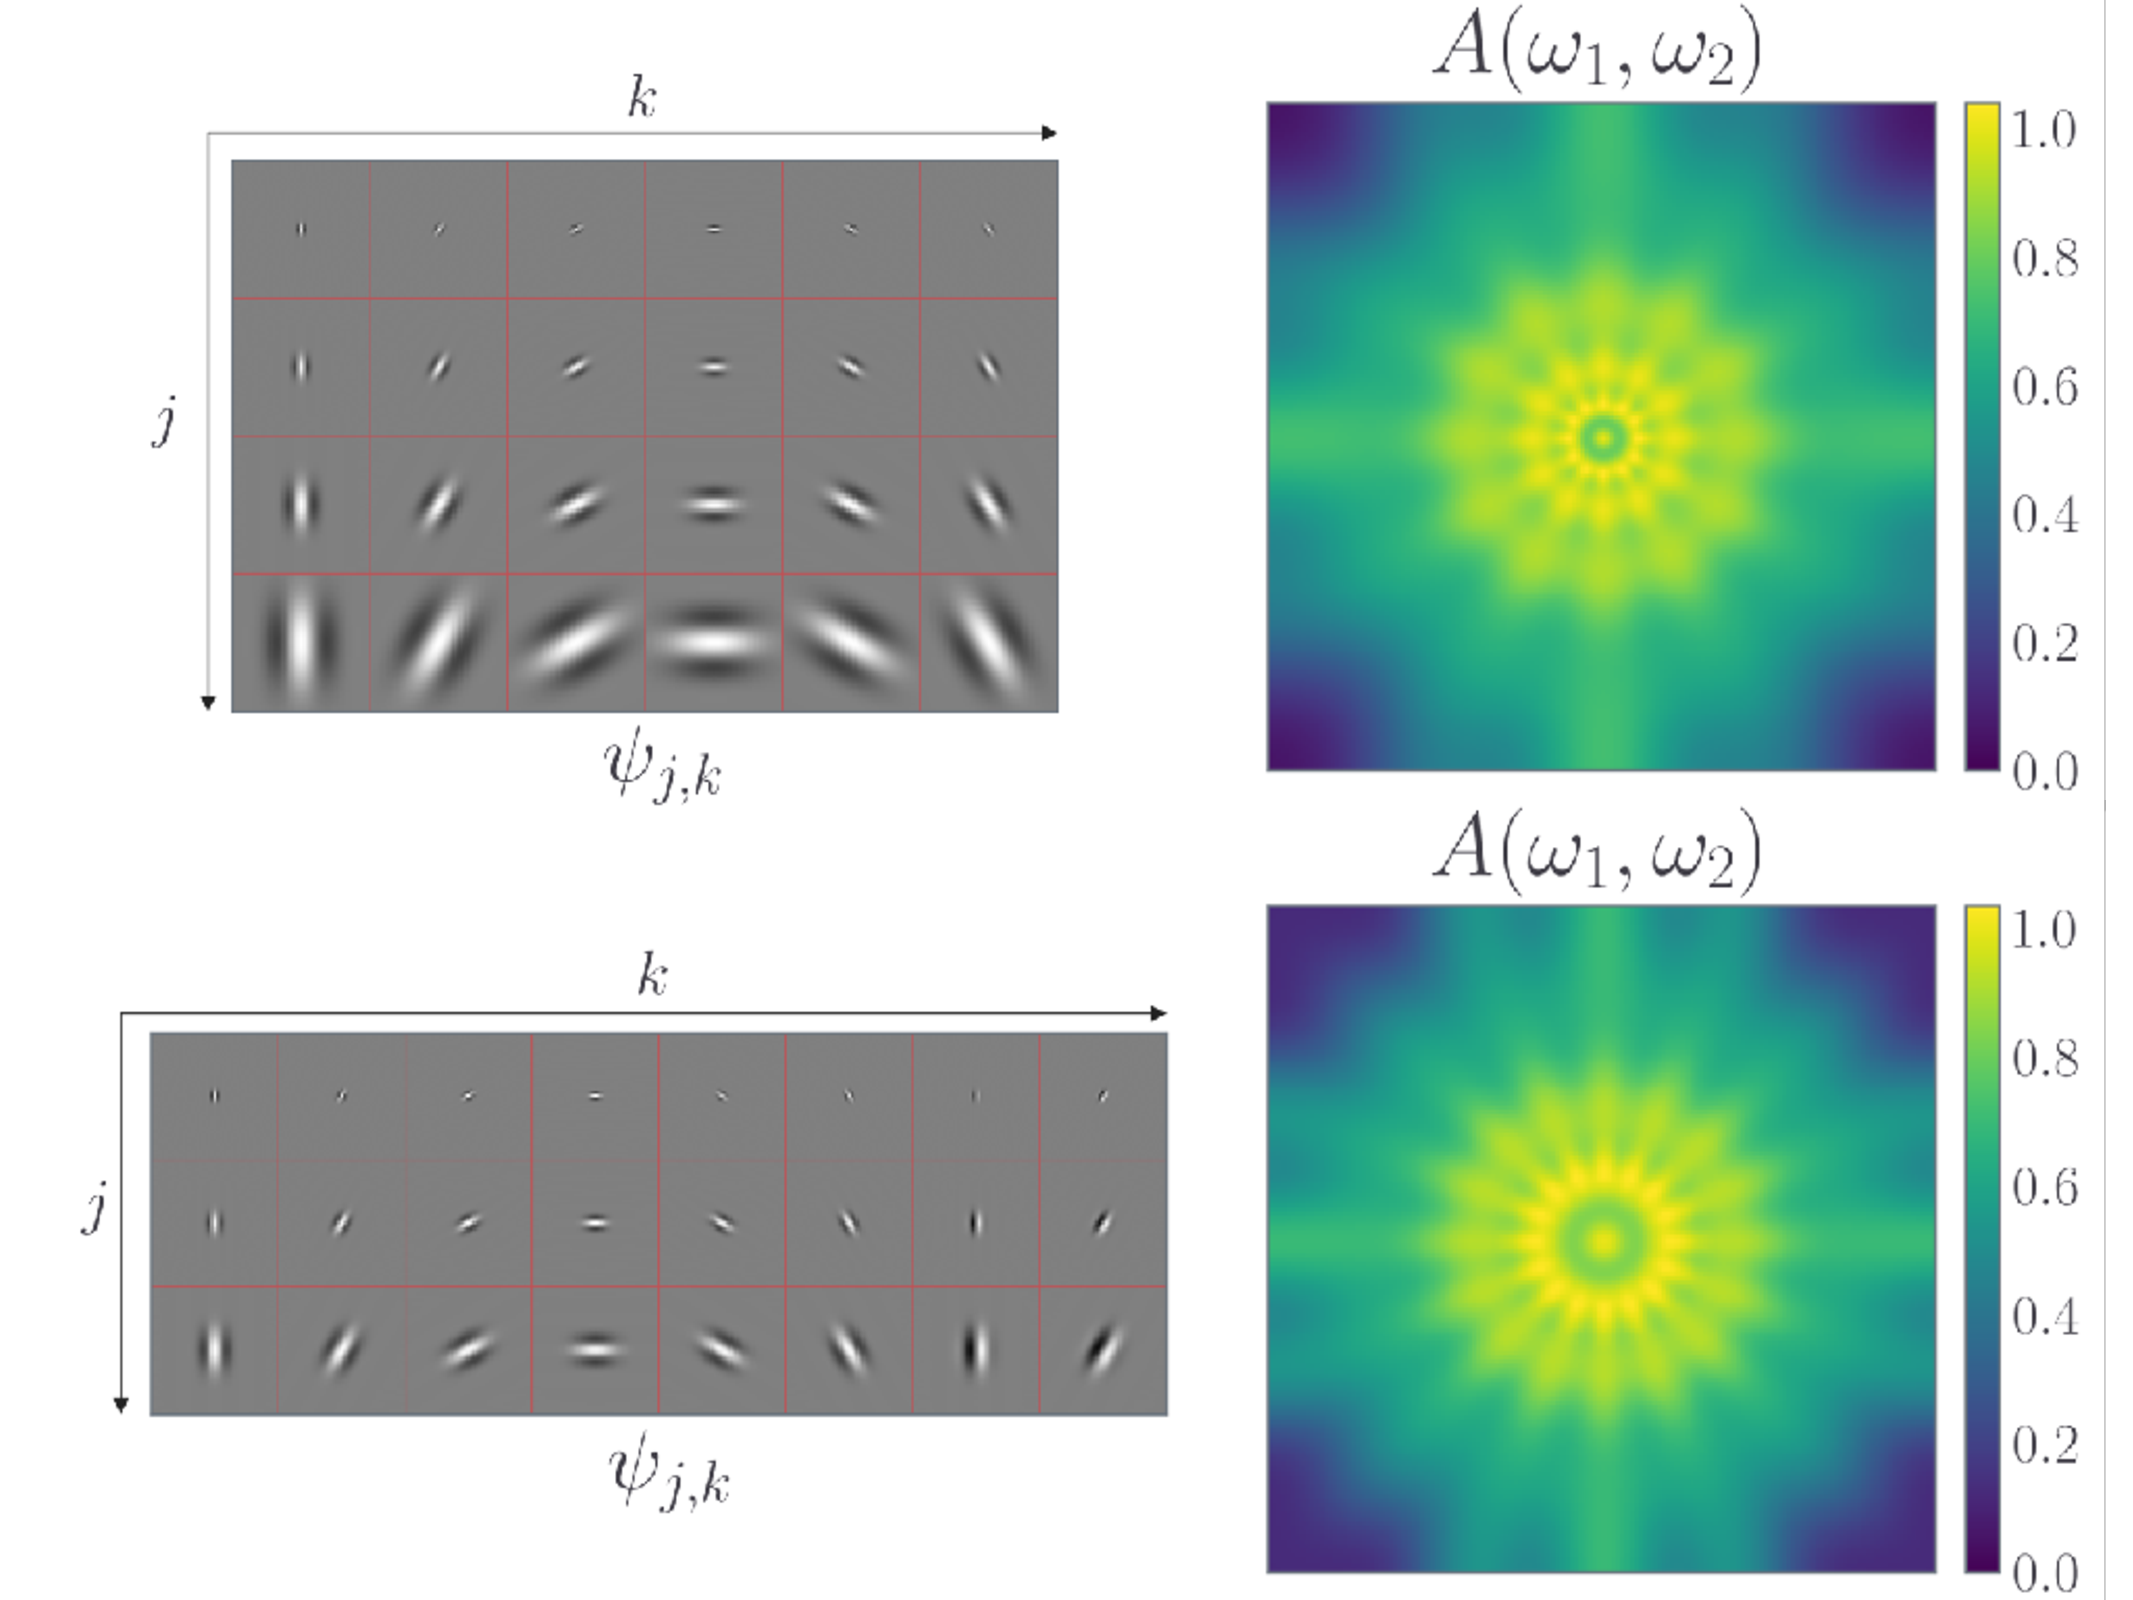
\includegraphics[width=1.1\textwidth]{\imgpath/im.pdf}
      }
    \mycaption{Two Morlet wavelet families and their tiling of the frequency
            plane}{For each set of parameters, the point spread functions of
            the \emph{real} wavelet bases are shown, next to their coverage of the
            frequency plane $A(\ww)$. Each square is $45\x 45$ pixels. Top:
            $J=3,\ K=6,\ Q=1$, Bottom: $J=4,\ K=8, Q=1$. None of the
            configurations cover the corners of the
            frequency plane, but this is often mostly noise.
            Increasing $J$, $K$ or $Q$ gives better frequency localization but at the
            cost of spatial localization and added complexity. Image is adapted
            from \cite{sifre_rigid-motion_2014-1}.}
      \label{fig:ch2:morlet_littlewood_paley}
  \end{figure}

The tightness of the frame is determined by the sampling grid of our wavelets
parameters $(\bmu{b}, a, \theta)$.
Common choices for sampling grids for 2-D wavelets are \cite[Section
2.2]{antoine_two-dimensional_2004}:
\begin{itemize}
  \item For dilations, $a = 2^{j/Q}$ for $j\in \mathbb{Z}$
    controlling the scale and $Q$, the number of scales per octave.
  \item For rotations, subdivide the interval $[0, \pi)$ into $K$ sections,
    and choose $\theta_k = \frac{k\pi}{K},\ k = \{0, 1, \ldots K-1\}$.
  \item For the translations, set the offsets $\bmu{b} =
    (l2^{j/Q},\ m2^{j/Q}),\ l,m \in \integers$.
\end{itemize}

  % If it ever exceeds 1, then there is overlap between bases.
  % Both of these conditions make invertibility difficult\footnote{In practise,
  % if $A(\ww)$ is only slightly greater 1 for only a few small areas of
  % $\ww$, approximate inversion can be achieved}.
  % The Fourier transform of the inverse
  % filters are defined by:
  % \begin{align}
    % \mathcal{F}\phiod_J^{-1}(\omega) &= A(\omega)^{-1} \mathcal{F}\phiod_J(\omega) \\
    % \mathcal{F}\psi_{\lambda}^{-1}(\omega) &= A(\omega)^{-1}
      % \mathcal{F}\psi_{\lambda}(\omega)
  % \end{align}

% The discrete wavelet transform (DWT) provides a non-redundant representation
  % of

% signals, hence overcomes the problem of redundancy. The DWT samples the
% timefrequency
% plane and only preserves the least number of the discrete coefficients
% that are required for perfect synthesis. The scale parameter a is sampled first
% on a logarithmic grid, and then the time parameter b is sampled with respect to
% the scale parameter. Though any sampling rate is possible, the DWT is mostly
% computed on the dyadic grid such that the DWT can be efficiently implemented
% by filter bank trees. This is of real value for practical applications.
% Figure 3.1 shows the diagram for a 4-level forward and inverse DWT, which
% explains how the DWT can be efficiently implemented by octave-band,
% discretetime
% filter bank trees. The notations in the diagram have the following meanings:
% 1. x is the original signal
% 2. ˆx is the reconstructed signal
% 3. H0 is the low-pass decomposition filter
% 4. H1 is the high-pass decomposition filter
% 5. °#2 is the operation that downsamples the signal by 2
% 6. G0 is the low-pass reconstruction filter
% 7. G1 is the high-pass reconstruction filter
% 8. °"2 is the operation that upsamples the signal by 2 by inserting zeros
% 9. w(j) are the wavelet coefficients in the j-th subband.
% The decomposition filter (H0, H1) and reconstruction filters (G0, G1) are
% carefully
% chosen in order that the wavelet transform can be inverted, i.e. x = ˆx. The
% above procedure can be represented by matrix-vector notations, which will later
% be introduced in 3.2.3.
%
\subsection{The $\DTCWT$}
  The $\DTCWT$ was first proposed by \citeauthor{kingsbury_dual-tree_1998} in
  \cite{kingsbury_dual-tree_1998, kingsbury_dual-tree_1998-1} as a way to combat
  many of the shortcomings of the DWT such as its poor directional
  selectivity and its poor shift-invariance. A thorough analysis of the
  properties and benefits of the $\DTCWT$ is done in
  \cite{kingsbury_image_1999,selesnick_dual-tree_2005}. Building on these
  properties, it been used
  successfully for denoising and inverse problems \cite{rivaz_bayesian_2001,
  zhang_bayesian_2008, zhang_variational_2015, miller_image_2008}, texture
  classification \cite{hatipoglu_texture_1999, rivaz_complex_1999}, image
  registration \cite{loo_motion-estimation-based_2001, chen_efficient_2012}
  and SIFT-style keypoint generation matching \cite{fauqueur_multiscale_2006,
  anderson_determining_2005, anderson_rotation-invariant_2006,
  bendale_multiscale_2010, ng_robust_2012} amongst many other applications.
  Compared to Gabor (or Morlet) image analysis, the authors of
  \cite{selesnick_dual-tree_2005} sum up the dangers as:
  \begin{quote}
    A typical Gabor image analysis is either expensive to compute, is
    noninvertible, or both.
  \end{quote}
  This nicely summarises the difference between this method and the Fourier
  based method outlined in \autoref{sec:ch2:morlet_fourier}. The $\DTCWT$ is
  a filter bank (FB) based wavelet transform. It is faster
  to implement than the Morlet analysis, as well as being more readily invertible.

\subsubsection{Design Criteria for the $\DTCWT$}
  As in \autoref{sec:ch2:complex_wavelets}, we want to have a complex mother
  wavelet $\psiod_c = \psiod_r + j\psiod_i$ and complex scaling function $\phiod_c =
  \phiod_r + j\phiod_i$, but now achieved with filter banks. The complex component
  allows for support of both the wavelet and scaling functions on only one half of
  the frequency plane.

  The dual-tree framework shown in \autoref{fig:ch2:dtcwt_1d_fb} can achieve this
  by making the real and imaginary components with their own DWT.
  We define:
  \begin{itemize}
    \item $h_0, h_1$ the low and high-pass analysis filters for $\phiod_r, \psiod_r$
    \item $g_0, g_1$ the low and high-pass analysis filters for $\phiod_i, \psiod_i$
    \item $\tilde{h}_0, \tilde{h}_1$ the low and high pass synthesis filters
      for $\tilde{\phiod}_r, \tilde{\psiod}_r$.
    \item $\tilde{g}_0, \tilde{g}_1$ the low and high pass synthesis filters for
      $\tilde{\phiod}_i, \tilde{\psiod}_i$.
  \end{itemize}

  The dilation and wavelet equations for a 1D filter bank implementation are
  \cite{selesnick_dual-tree_2005}:
  \begin{align}
    \phiod_r(t) & =  \sqrt{2} \sum_n h_0(n) \phiod_r(2t-n) \\
    \psiod_r(t) & =  \sqrt{2} \sum_n h_1(n) \phiod_r(2t-n) \\
    \phiod_i(t) & =  \sqrt{2} \sum_n g_0(n) \phiod_i(2t-n) \\
    \psiod_i(t) & =  \sqrt{2} \sum_n g_1(n) \phiod_i(2t-n)
  \end{align}

  \begin{figure}
    \centering
      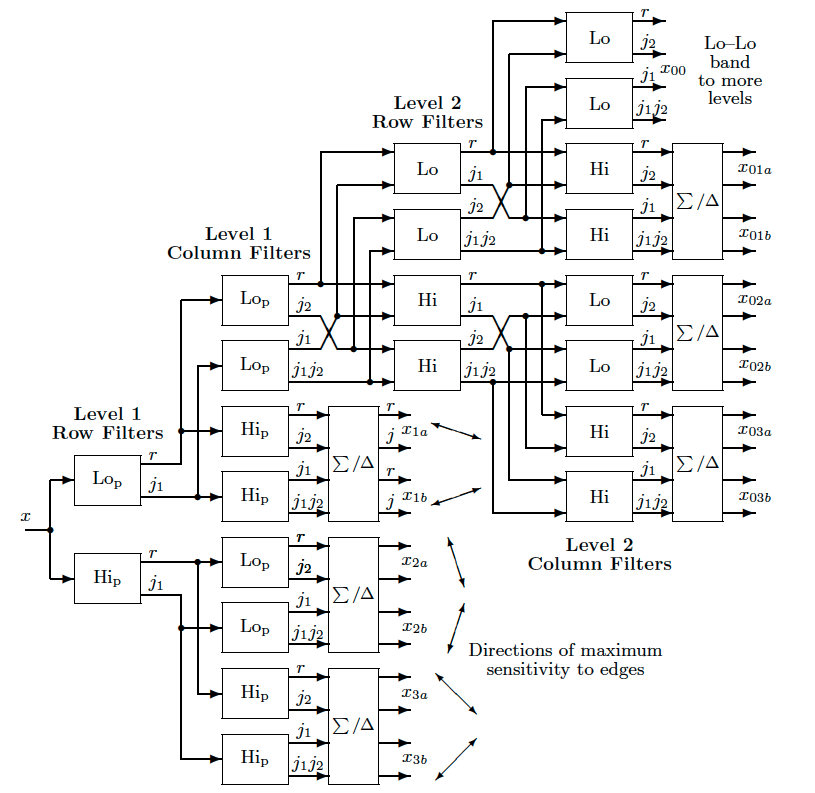
\includegraphics[width=\textwidth]{\imgpath/dtcwt_fb.png}
      \mycaption
      {Analysis FBs for the 1-D $\DTCWT$}{Top `tree' forms the real component of the
      complex wavelet $\psiod_r$, and the bottom tree forms the imaginary (Hilbert
      pair) component $\psiod_i$. Image is taken from
      \cite{kingsbury_image_1999}.}
      \label{fig:ch2:dtcwt_1d_fb}
  \end{figure}

  Designing a filter bank implementation that results in Hilbert-symmetric
  wavelets does not appear to be an easy task. However, it was shown
  by \citeauthor{kingsbury_image_1999} in \cite{kingsbury_image_1999} (and later proved by
  \citeauthor{selesnick_hilbert_2001} in \cite{selesnick_hilbert_2001}) that the
  necessary conditions are conceptually very simple. One low-pass filter must be
  a \emph{half-sample shift} of the other. I.e., if $g_0(n) = h_0(n-1/2)$ then
  the corresponding wavelets are a Hilbert transform pair
  \begin{equation}
    \psiod_g(t) \approx \mathcal{H}\{\psiod_h(t)\}
  \end{equation}
  As the $\DTCWT$ is designed as an invertible filter bank implementation, this
  is only one of the constraints. As with conventional (real) discrete wavelets,
  there are also perfect reconstruction, finite support, linear phase and
  vanishing moment constraints to consider in the filter bank design.

  The derivation of the filters that meet these conditions is covered in
  detail in \cite{kingsbury_complex_2001, kingsbury_design_2003}, and in
  general in \cite{selesnick_dual-tree_2005}. The result is the
  option of three main families of filters: biorthogonal filters ($h_0[n] =
  h_0[N-1-n]$ and $g_0[n] = g_0[N-n]$), q-shift filters ($g_0[n]
  = h_0[N-1-n]$), and common-factor filters.

\subsubsection{2-D $\DTCWT$ and its Properties}
  While analytic wavelets in 1D are useful for their shift-invariance, the real
  beauty of the $\DTCWT$ lies in its ability to make a separable 2-D wavelet
  transform with oriented wavelets.

  \autoref{fig:ch2:dwt_hh} shows the spectrum of
  the wavelet when the separable product uses purely real wavelets, as is the
  case with the DWT\@. \autoref{fig:ch2:dtcwt_hh} however, shows the separable
  product of two complex, analytic wavelets resulting in a localized and
  oriented 2-D wavelet.

  Note that in this thesis, we name the wavelets by the direction of the edge
  that they are most sensitive to.
  For example, the $135\degs$ is the second image in \autoref{fig:ch2:dtcwt_wavelets} and
  can be obtained by the separable product:
  \begin{align}
    \psitd(\xy) &= \psiod_c(u_1) \psiod_c^*(u_2) \label{eq:ch2:wavelet_separable_product}\\
              &= \left(\psiod_r(u_1) + j\psiod_i(u_1)\right)
                 \left(\psiod_r(u_2) - j\psiod_i(u_2)\right) \\
              &= \left(\psiod_r(u_1)\psiod_r(u_2) + \psiod_i(u_1)\psiod_i(u_2)\right)
                +j \left(\psiod_r(u_1)\psiod_i(u_2) - \psiod_i(u_1)\psiod_r(u_2)\right)
                \label{eq:ch2:dtcwt_2d_product}
  \end{align}
  Similar equations can be obtained for the other five wavelets and the scaling
  function, by replacing $\psiod$ with $\phiod$ for each direction in turn (but not both
  together), and not taking the complex conjugate
  in \eqref{eq:ch2:wavelet_separable_product} to get the filters in the
  right-hand half of the frequency plane. The 2-D $\DTCWT$ requires four 2-D
  DWTs to calculate the four possible combinations of real and imaginary
  components. The high and lowpass outputs from these DWTs can then be summed in
  different ways as in \eqref{eq:ch2:dtcwt_2d_product} to get the complex
  bandpass wavelets. \autoref{fig:ch2:dtcwt_wavelets} shows the resulting
  wavelets both in the spatial domain and their idealized support in the
  frequency domain.

  \begin{figure}
%      \centering
      \subfloat[]{\makebox[\textwidth][c]{%
        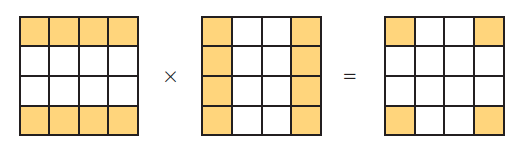
\includegraphics[width=0.6\textwidth]{\imgpath/dwt_hh.png}
        \label{fig:ch2:dwt_hh}}}
      \newline
      \subfloat[]{\makebox[\textwidth][c]{%
        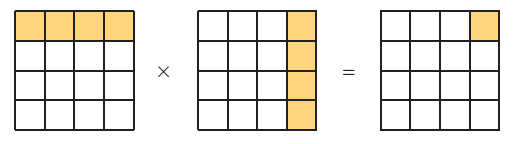
\includegraphics[width=0.6\textwidth]{\imgpath/dtcwt_hh.png}
        \label{fig:ch2:dtcwt_hh}}}
      \mycaption{The DWT high-high vs the $\DTCWT$ high-high frequency support}
              {\subref{fig:ch2:dwt_hh} The high-high DWT wavelet having a passband in
              all 4 corners of the frequency plane vs \subref{fig:ch2:dtcwt_hh} the
              high-high $\DTCWT$ wavelet frequency support only existing in one
              quadrant. Figure is taken from \cite{selesnick_dual-tree_2005}}
      \label{fig:ch2:dwt_dtcwt_hh}
  \end{figure}
  \begin{figure}
    \centering
      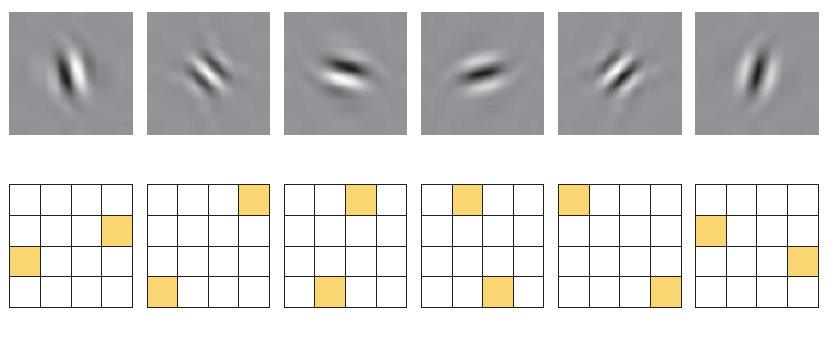
\includegraphics[width=\textwidth]{\imgpath/dtcwt_wavelets.png}
    \mycaption{Wavelets from the 2-D $\DTCWT$}{\textbf{Top:} The six  oriented filters
      in the space domain (only the real wavelets are shown). From left to right
      these are the $105\degs, 135\degs, 165\degs, 15\degs, 45\degs, 75\degs$
      wavelets. \textbf{Bottom:}
      Idealized support of the Fourier spectrum of each wavelet in the 2-D
      frequency plane. Spectra of the real wavelets are shown --- the
      spectra of the complex wavelets ($\psiod_r + j\psiod_i$) only has support in the top
      half of the plane. Figure is taken from \cite{selesnick_dual-tree_2005}.}
      \label{fig:ch2:dtcwt_wavelets}
  \end{figure}

  \subsubsection{Tightness and Invertibility}\label{sec:ch2:dtcwt_tight}
  We analysed the coverage of the frequency plane for the Morlet wavelet family
  and saw what areas of the spectrum were better covered than others. How about
  for the $\DTCWT$?

  It is important to note that in the case of the q-shift $\DTCWT$, the wavelet
  transform is also approximately unitary, i.e.,\
  \begin{equation}
    \norm{x}^2 \approx \norm{\mathcal{W}x}^2
  \end{equation}
  and the implementation is perfectly invertible as $A(\ww)$ from
  \eqref{eq:ch2:lwood_paley}
  function is unity (or very near unity) $\forall \ww \in [-\pi, \pi]\x [-\pi,
  pi]$. This is not a surprise, as it is a design
  constraint in choosing the filters, but is nonetheless important to note.

  % A beneficial property of energy conservation is that the noise in the input
  % will equal the noise in the wavelet coefficients. When we introduce
  % Scatternets, we can show that we can keep the unitary property in the
  % scattering coefficients.
  % This is an important property, particularly in light
  % of the recent investigations in \cite{szegedy_intriguing_2013}. This paper
  % saw that it is easy to find cases in CNNs where a small amount of input
  % perturbation results in a completely different class label (see
  % \autoref{fig:ch2:difference}). Having a unitary transform limits the
  % amount the features can change, which will make the entire network more
  % stable to distortion and noise.

  % \begin{figure}
    % % \subfloat{\makebox[0.6\textwidth][c]{%
      % % 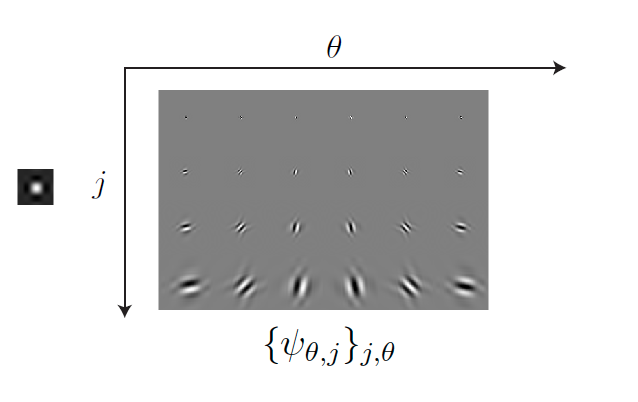
\includegraphics[width=0.7\textwidth,valign=c]{\imgpath/dtcwt_real_4scales.png}
    % % }}
    % % \subfloat{\makebox[0.4\textwidth][c]{%
      % % 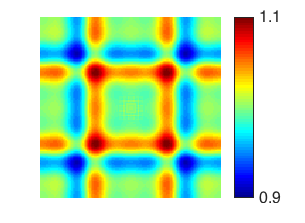
\includegraphics[width=0.5\textwidth,valign=c]{\imgpath/dtcwt_lwoodpaley_2.png}
    % % }}
    % 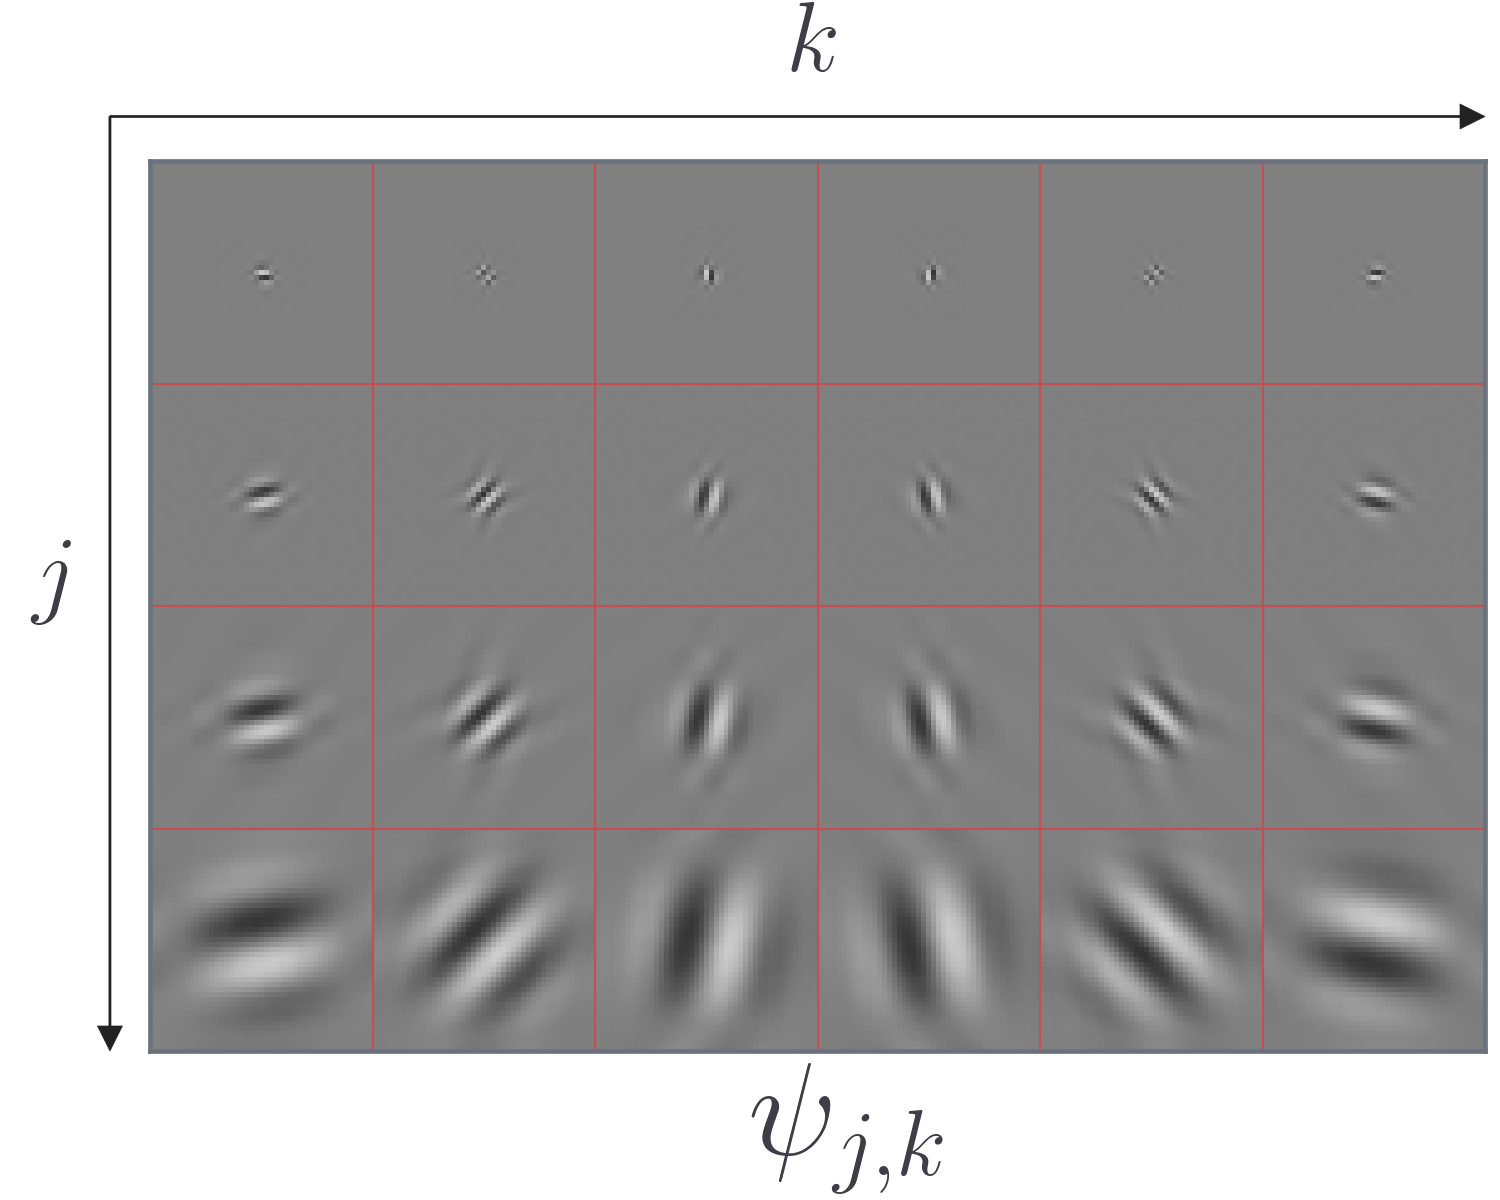
\includegraphics[width=0.8\textwidth]{\imgpath/dtcwt_j4k6.png}
    % \mycaption{$\DTCWT$ family for $J=4$ and their frequency coverage}{}
    % \label{fig:ch2:dtcwt_lwoodpaley}
  % \end{figure}

\subsection{Summary of Methods}
  One final comparison to make between the $\DTCWT$ and the Morlet wavelets is
  their frequency coverage. The Morlet wavelets have flexibility at the cost of
  computational expense and can be made to have tighter angular resolution than
  the $\DTCWT$. However it is not always
  better to keep using finer and finer resolutions, indeed the Fourier
  transform gives the ultimate in angular resolution but as mentioned, this
  makes it less stable to shifts and deformations. We will explore this in more
  depth in Chapter 3.

  % \autoref{tab:dtcwt_vs_dwt_vs_mallat} compares the advantages and
  % disadvantages of the wavelet methods discussed in this chapter.
  % \begin{figure}
    % \subfloat[$\DTCWT$ wavelets (left to right) --- $15\degs$, $45\degs$ and $75\degs$]{%
      % \makebox[\textwidth][c]{%
      % 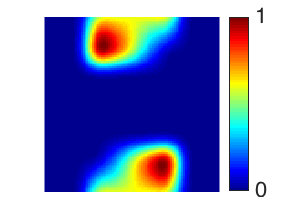
\includegraphics[width=0.4\textwidth]{\imgpath/dtcwt_15deg_energy.png}
      % 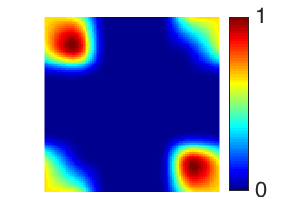
\includegraphics[width=0.4\textwidth]{\imgpath/dtcwt_45deg_energy.png}
      % 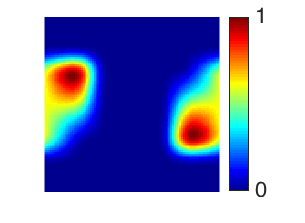
\includegraphics[width=0.4\textwidth]{\imgpath/dtcwt_75deg_energy.png}
    % }}
    % \newline
    % \subfloat[Morlet wavelets (left to right) --- $0\degs$, $45\degs$, $90\degs$]
      % $67.5\degs$,  and $90\degs$]{%
      % \makebox[\textwidth][c]{%
      % 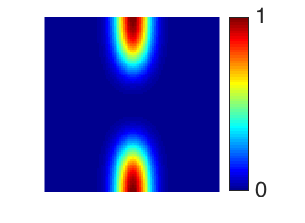
\includegraphics[width=0.4\textwidth]{\imgpath/mallat_0deg_energy.png}
      % 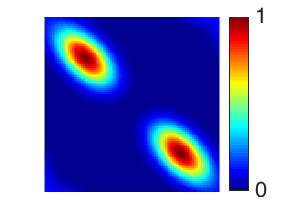
\includegraphics[width=0.4\textwidth]{\imgpath/mallat_45deg_energy.png}
      % 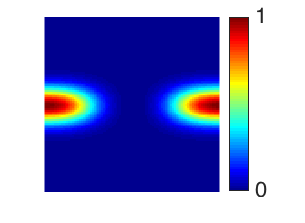
\includegraphics[width=0.4\textwidth]{\imgpath/mallat_90deg_energy.png}
    % }}
    % \newline
    % \subfloat[]{%
      % % Use two makebox commands to center the images
      % \makebox[0.5\textwidth][c]{%
        % \hspace{1cm}
        % 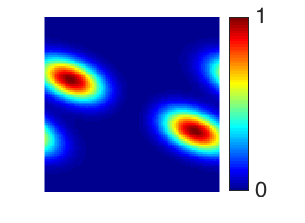
\includegraphics[width=0.4\textwidth,center]{\imgpath/mallat_675deg_energy.png}
      % }
      % \makebox[0.5\textwidth][c]{%
        % \hspace{-1cm}
        % 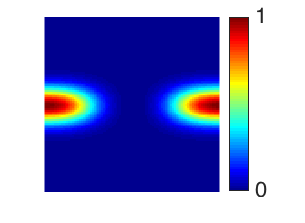
\includegraphics[width=0.4\textwidth,center]{\imgpath/mallat_90deg_energy.png}
      % }
    % }
    % \mycaption{Comparison of the energy spectra for $\DTCWT$ wavelets to Morlet
    % wavelets}{Normalized Energy spectra of the $\DTCWT$ wavelets versus the preferred
          % 8 orientation Morlet wavelets by Mallat for the second quadrant.
          % Orientations listed refer to the edge orientation in the spatial
          % domain that gives the highest response. All wavelets have been
          % normalized to be between zero and one.
          % The Morlet wavelets have finer angular
          % resolution, which can give better discrimination, at the cost of
          % decreasing stability to deformations, and requiring larger spatial
          % support.}
    % \label{fig:ch2:wavelet_freq_resp}
  % \end{figure}
